\documentclass[11pt]{article}
\usepackage[a4paper,margin=25mm]{geometry}
\usepackage{amsmath,amssymb,amsthm}
\usepackage{booktabs}
\usepackage{graphicx}
\usepackage{hyperref}
\usepackage{natbib}
\usepackage{xcolor}
\usepackage{tikz}
\usepackage{pgfplots}
\pgfplotsset{compat=1.18}
\usepgfplotslibrary{groupplots}
\newtheorem{proposition}{Proposition}
\newtheorem{theorem}{Theorem}
\newtheorem{definition}{Definition}
\newcommand{\todo}[1]{\textcolor{red}{[#1]}}
\newcommand{\cov}{\mathrm{cov}}
% Placeholder for a figure the authors insert by hand: a framed box with the
% word "image" and, in the caption, what the figure must show.
\newcommand{\imageplaceholder}[2]{\fbox{\parbox[c][#2][c]{#1}{\centering\Large\textsf{image}}}}

\title{A Certificate That Survives the Search:\\
Subgroup Discovery on One Grid with Partial-Axis Centres}
\author{Gleb Nezhdanov \and Thinzar Aung Win \todo{affiliations; author order}}
\date{Draft of \today}

\begin{document}
\maketitle

\begin{abstract}
Subgroup discovery returns overlapping conjunctive rules chosen by reading the target, so a confidence statement computed for one rule as if fixed in advance is invalid.
We study the version of the problem in which every group is a cell of one grid spanned by at most four columns, and measure what the constraint is worth.
Its main return is a certificate that survives the search: the cells of all such grids form a family fixed before the target is read, so a cell whose target count reaches a heterogeneous-binomial threshold at level $\alpha/T$, $T$ the number of distinct row sets in the family, is certified with family-wise error $\alpha$, for every purity floor $\tau$ at once and whatever rule chose the grid. No decision tree has such a family; the exploratory/holdout split certifies any method, but on the same folds it certifies on average a quarter less coverage, and what it certifies holds $\tau$ on held-out rows half as often.
The constraint's cost is coverage, paid for fixing every axis rather than for sharing columns: a centre that leaves some axes free (a \emph{partial-axis centre}) recovers, under the certificate, the coverage of free disjoint rules on every table but the widest of seventeen, matches an optimal depth-4 tree with the same objective, and names fewer than half the columns of the free rules (3.9 against 8.3 at budget 32); the certificate is unchanged.
The usual overlapping-rule baseline is not like for like: its unions fall below $\tau$ on held-out rows in 40\,\% of the splits.
\end{abstract}

\section{Introduction}

A data analyst asks where a value of a categorical target lives. Subgroup discovery~\citep{klosgen1996,wrobel1997,atzmueller2015} answers with a ranked list of conjunctions $c_1 = v_1 \wedge \dots \wedge c_\ell = v_\ell$. Three properties of such a list limit what can be said about it. The rules were chosen by reading the target, so a confidence statement computed for one rule as if it had been fixed in advance is invalid; the standard remedies, a Bonferroni correction over the whole description language or a holdout half (both in~\citealp{webb2007}), either pay for every conjunction the language can express or give up half the rows. The rules overlap, so the purity of two rules says nothing about the purity of their union. And the rules use different columns, so the description of where the target lives is as long as the list.

The approach studied here fixes the description language first. A \emph{schema} is a set $S$ of at most four columns; the \emph{grid} on $S$ is the joint partition of the rows by the values of those columns; a \emph{centre} is a cell of purity at least $\tau$ with at least $m$ rows. The cells of every schema of size $\le4$ form a family that depends on the columns alone, and that family, not the description language, is what a post-selection certificate has to pay for; the centres of one schema are cells of one partition, hence disjoint; and a schema names at most four columns. A schema with its centres is also one display (a table, a cube, or a cube with a fourth axis stepped through), which is where the constraint came from, but nothing below depends on the display. The search is exhaustive over schemas of every size up to four, so it can find pairs of columns that are jointly informative while neither is alone, which a greedy chain cannot~\citep{krause2005}. The software (VSF) shows the winning schema as a lattice with the centres coloured (in its partial mode, partial centres as lines through their member cells), every scored schema as a point in a coverage landscape, and the cells of the winners as a filtered rule list; this paper is about the search and its guarantees, not the display.

Two questions decide whether this is a method or merely a constraint that costs coverage:

\begin{enumerate}
\item \textbf{Is anything shown still true after the search?} The best of $\sum_{d\le 4}\binom{M}{d}$ schemas was chosen by looking at the target; a purity certificate computed for one schema alone is invalid after that choice. What does a certificate that survives the choice cost, and how does it compare with the alternatives a rule list or a tree can have?
\item \textbf{What does one grid cost?} At an equal budget of conditions, how much target coverage does the one-grid constraint lose against free rules and against an optimal tree, and what mechanism loses it?
\end{enumerate}

\paragraph{Contributions.}
\begin{enumerate}
\item \emph{A certificate that survives the search.} A cell is certified when its target count reaches $k^*(n,\tau,\alpha/T)$, a heterogeneous-binomial threshold with $T$ the number of distinct row sets among all cells the search can display. The guarantee is a union bound, valid for any rule of schema choice and any dependence between cells, and holds simultaneously for every $\tau$ (Section~\ref{sec:certificate}). Its price is computed exactly (the smallest certifiable cell as a function of $T$, $\tau$ and the margin above $\tau$) and compared, on the same folds, with the exploratory/holdout split, which certifies a quarter less and holds on held-out rows half as often. No tree, greedy or optimal, and no rule list fitted to the target (SSD++) has a family fixed before the target is read. Free conjunctive rules can be certified, but only through this family: every rule of length $\le4$ is a cell of one of the grids, so the certificate they inherit is the grid's (Section~\ref{sec:protocol}).
\item \emph{Partial-axis centres.} We relax the grid constraint by one step: a centre may fix a subset $S'\subset S$ of the schema's axes. Its candidates are cells of sub-schemas the search already enumerates, so $T$ and the certificate are unchanged; a deterministic disjoint packing keeps coverage a sum and keeps the purity claim for the union. The relaxation removes most of the price of the one-grid constraint (Section~\ref{sec:results}), shows where the price came from --- fixing all axes, not sharing the columns (Section~\ref{sec:mechanism}) --- and leaves the certified method level with free disjoint rules on every table but the widest, and with an optimal depth-4 tree, on coverage (Sections~\ref{sec:mechanism} and~\ref{sec:treeopt}), with fewer conditions and fewer than half the columns of the free rules (Section~\ref{sec:compact}).
\item \emph{An evaluation protocol and the baselines it needs.} Nested cross-validation with the encoding (capacity rule, level merging, family size) fitted on the training fold; held-out purity of the \emph{union} of selected groups; a disjoint-rule baseline, since budgeted maximum coverage over overlapping rules yields unions below $\tau$ in half of the held-out splits; an optimal tree with class weights $1:\tau/(1-\tau)$, which makes the weighted error the purity-constrained objective exactly; and WRAcc lists with and without the purity floor (Section~\ref{sec:protocol}).
\end{enumerate}

What we do not claim: that one grid covers more than free rules or than an optimal tree (it does not; the tree is ahead on net coverage and more compact), or that the shared picture is easier to read than a list (we have not measured it, and no result below depends on it). What the grid is shown to buy is measured: a certificate that no tree and no target-fitted rule list has (Section~\ref{sec:certificate}), coverage level with the best of them under it (Sections~\ref{sec:mechanism}, \ref{sec:treeopt}), a union whose held-out purity holds $\tau$ where that of overlapping rules does not (Section~\ref{sec:mechanism}), and a description with fewer columns than free rules at the same coverage (Section~\ref{sec:compact}).

\section{Related work}\label{sec:related}

\paragraph{Subgroup discovery.} Subgroup discovery~\citep{klosgen1996,wrobel1997,herrera2011,atzmueller2015} finds descriptions of row sets with an unusual target distribution. SD-Map~\citep{atzmueller2006}, CN2-SD~\citep{lavrac2004}, beam and best-first search in pysubgroup~\citep{lemmerich2018}, diverse top-$k$ (DSSD,~\citealp{vanleeuwen2012}), MDL-based rule sets and lists~\citep{fischer2019,proenca2022}. Redundancy among top-$k$ subgroups is the problem DSSD and the MDL methods address; the one-grid constraint addresses it structurally, since disjoint cells of one partition cannot overlap. Quality functions are typically size$\times$lift (WRAcc); the task here, maximum coverage subject to a purity floor, is a different objective, and on \texttt{titanic} a WRAcc-ranked list from pysubgroup (Apriori, depth $\le4$) puts \texttt{sex = female} first (purity 0.73) and at $\tau=0.9$ never reaches $\tau$ in any held-out split; with the $\tau$ filter applied it is the same candidate family as free rules in a different order, one that costs coverage against budgeted maximum coverage and gains held-out purity. Section~\ref{sec:wracc} runs both lists, with and without the filter, as baselines (\texttt{wracc}, \texttt{wracc\_raw}).

\paragraph{Statistically sound pattern mining.} Bonferroni over the pattern space~\citep{webb2007}, LAMP and Tarone's trick~\citep{terada2013,llinares2015}, the two-sample split (exploratory/holdout,~\citealp{webb2007}), and the tutorial of~\citet{hamalainen2019} on which corrections are valid after a search. The recent line of resampling-based methods --- Westfall--Young permutation with pruning~\citep{llinares2015}, unconditional tests (SPuManTE,~\citealp{pellegrina2019}), the most significant patterns by permutation~\citep{pellegrina2020}, and few-shot resampling with supremum-deviation bounds (FSR,~\citealp{pellegrina2024}; FewRS,~\citealp{pellegrina2026}) --- controls the family-wise error far more efficiently than a union bound, but for a different null: every one of them tests whether a pattern's quality departs from what a target independent of the features would give, i.e.\ association. The certificate here bounds a one-sided \emph{level}, $\bar p_c\le\tau$, which a permutation null cannot address (Section~\ref{sec:certificate}: a cell of purity $0.85$ is extreme against independence and would be ``certified'' as $>0.9$). Our certificate is of the Bonferroni family with the family taken over row sets rather than descriptions, with a threshold valid for heterogeneous rows~\citep{hoeffding1956}; Tarone's improvement is available only at a fixed $\tau$ and is not used for the interactive setting. Statistical control of \emph{subgroup} selection in the clinical sense (a subgroup that benefits from treatment,~\citealp{schnell2023}) asks a related question with a treatment contrast in place of a purity floor.

\paragraph{Controlled visual exploration.} Controlling false discoveries during interactive exploration~\citep{zhao2017,zgraggen2018}; visual subgroup discovery in VIKAMINE~\citep{atzmueller2005}; intersectional subgroup analysis with significance in FairVis~\citep{cabrera2019}. Displays of cells of a multi-way table with area and colour go back to mosaic plots~\citep{friendly1994}. We do not claim novelty for the display; the claim is about the search and the certificate behind it.

\paragraph{Optimal trees and slice finding.} A depth-4 decision tree is the most natural competitor for a 4-column description; CART is greedy at the root and loses planted grid structure, while an optimal tree~\citep{lin2020,demirovic2022,aglin2020} is the stronger baseline: the solvers minimise misclassification, but with class weights $1:\tau/(1-\tau)$ the weighted error of a tree is, up to a constant, the negative of the net coverage of its positive leaves, so an optimal weighted tree is the optimal single partition for the purity-constrained objective (Section~\ref{sec:treeopt}). Slice Finder~\citep{chung2019} looks for underperforming slices of a model with the same conjunctive language.

\section{Problem and method}\label{sec:method}

\subsection{Setting}
Rows $i=1,\dots,N$ with categorical columns $X_{i1},\dots,X_{iM}$ (numeric columns are binned once, on all rows, and the bins are part of the dataset) and a binary target $z_i\in\{0,1\}$ with $P=\sum_i z_i$ positives. Purity floor $\tau$ above the base rate $P/N$, size floor $m$.

\begin{definition}[Grid, centre, coverage]
For a schema $S\subseteq\{1,\dots,M\}$, $|S|\le 4$, the grid $\mathcal{G}(S)$ is the partition of rows by the joint value of the columns in $S$, after the capacity rule of Section~\ref{sec:capacity}. A cell $c$ with $n_c$ rows and $k_c$ positives is a centre if $n_c\ge m$ and $k_c/n_c\ge\tau$ (observed-purity rule) or $k_c\ge k^*(n_c,\tau,\alpha/T)$ (certified rule, Section~\ref{sec:certificate}). The coverage of $S$ is $\cov(S)=\sum_{c\text{ centre}} k_c / P$.
\end{definition}

The full-grid search returns, for each $d\le 4$, $S^*_d=\arg\max_{|S|=d}\cov(S)$, ties broken by fewer centres, then smaller mass, then the best per-cell lower bound. Every $\binom{M}{d}$ subset is scored.

\subsection{Capacity rule and level merging}\label{sec:capacity}
A grid may occupy at most $\lfloor N/10\rfloor$ cells; when it does not fit, the widest column loses its rarest level into an ``other'' group, one level at a time, until it fits. The rule reads no target and is refitted on the training rows in every fold (Section~\ref{sec:protocol}). Levels of an ordered column are merged by adjacency, of a nominal column by frequency; the merge sequence is deterministic (widest column first, ties by column index) and the first state that fits is found by bisection over the step count. The rule bounds the number of cells the display has to draw and the number of hypotheses in the family; it also breaks the nesting of cells across dimensionalities (11.9\,\% of nested pairs on \texttt{titanic}), which is why an optimistic-estimate pruning of the search is not attempted here.

\subsection{Partial-axis centres}\label{sec:partial}
\begin{definition}[Partial-axis centre]
A partial-axis centre (\emph{partial centre} for short) of schema $S$ is a centre of the grid $\mathcal{G}(S')$ for some non-empty $S'\subseteq S$. It fixes $|S'|$ axes of $S$ and leaves $|S|-|S'|$ free; it costs $|S'|$ conditions. Geometrically it is a bar ($|S'|=|S|-1$), a plate, or a layer of the cube of $S$ (Figure~\ref{fig:mech}).
\end{definition}

The software draws a partial centre as a line through its member cells along the free axis, from the first to the last occupied cell (a lattice of such lines when two axes are free); a layer, which fixes only the axis that is stepped through, is reported in text rather than drawn; on request a centre collapses to one sphere on the wall of the cube at its projection, sized by its rows and coloured by its pooled purity, which is the cell the collapse of the free axis would produce.

Partial centres of different sub-schemas may overlap. We select a disjoint set by a deterministic greedy: candidates in the order (more positives, fewer conditions, fewer rows, enumeration order), each taken if it shares no row with those already taken. The coverage of $S$ with partial centres is then $\cov^{\mathrm{p}}(S)=\sum_{c\text{ chosen}}k_c/P\ \ge\ \cov(S)$, since every full cell is a candidate. The union of disjoint groups each of purity $\ge\tau$ has purity $\ge\tau$.

Three properties make the relaxation free. (i) The candidates of $S$ are the centres of its sub-schemas, which the exhaustive enumeration visits before $S$ ($d=1,\dots,4$ in order); nothing new is computed. (ii) Every candidate is a cell of a partition of some $S'$ with $|S'|\le4$, hence a member of the family $T$ of Section~\ref{sec:certificate}: the certificate is unchanged. (iii) The display is unchanged: a partial centre is a union of cells of the same cube. Figure~\ref{fig:example} shows one winning schema with its partial centres on a real table.

\begin{figure}[t]\centering
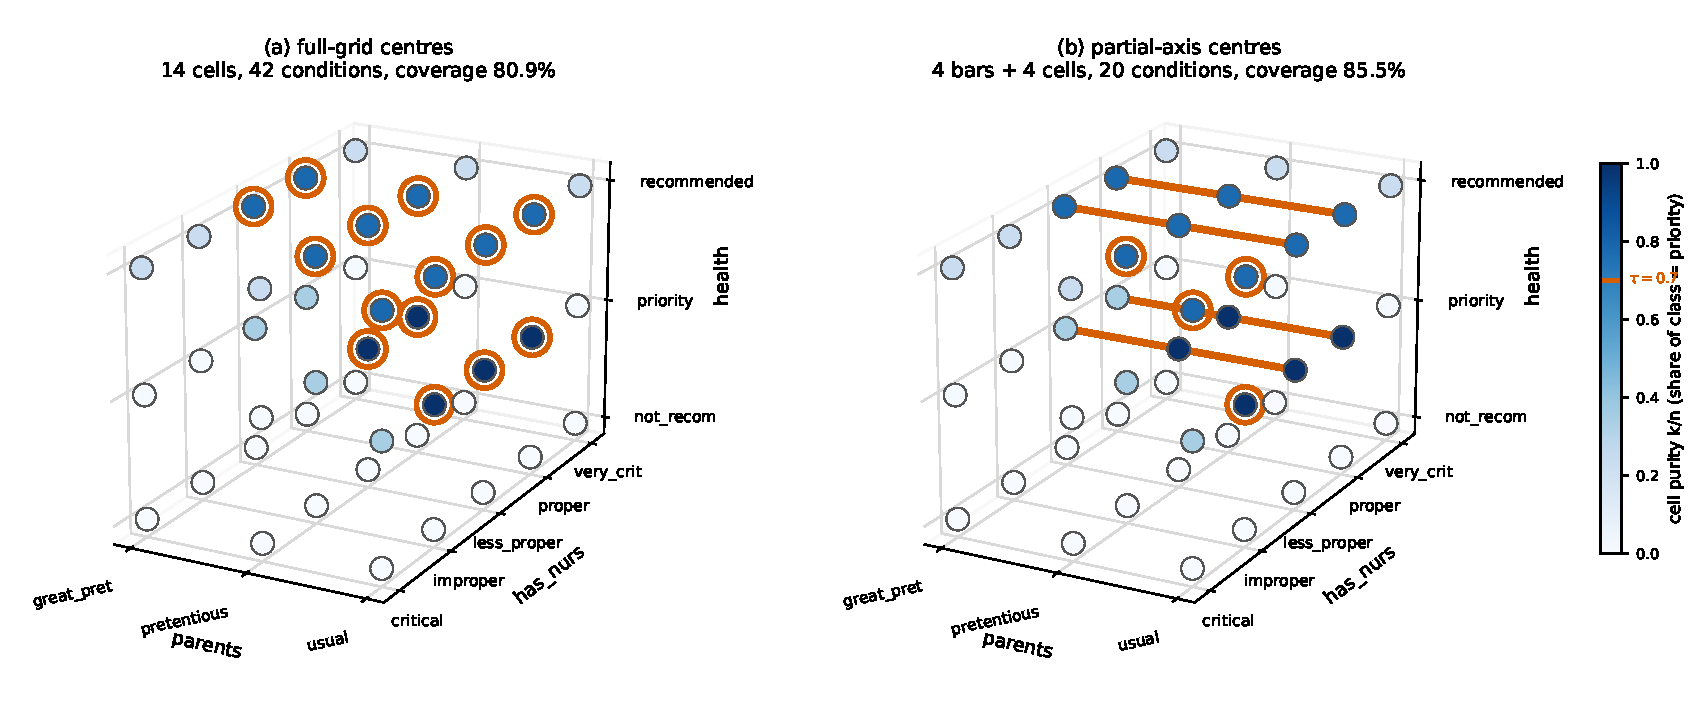
\includegraphics[width=\linewidth]{fig_example.pdf}
\caption{The winning three-column schema on \texttt{nursery} (target $\texttt{class}=\texttt{priority}$, $\tau=0.7$, $m=1$, all rows), drawn from the data by \texttt{experiments/fig\_example.py}. Spheres are the 45 occupied cells of the grid $\texttt{parents}\times\texttt{has\_nurs}\times\texttt{health}$, coloured by purity $k/n$ (single-hue scale; the mark on the bar is $\tau$). The software colours cells by three purity zones (above $\tau$, between the base rate and $\tau$, below); a continuous scale is used here so that the purity of each cell a bar pools is visible. Every cell has 288 rows, since the table is a full factorial design, so size encodes nothing. (a) The full grid: the 14 cells at purity $\ge\tau$, ringed, cover $80.9\,\%$ of the target rows for $42$ conditions. (b) Partial-axis centres of the same schema: four bars, each a cell of the sub-grid $\texttt{has\_nurs}\times\texttt{health}$ drawn as a line through its three member cells along the free axis \texttt{parents} (e.g.\ $\texttt{has\_nurs}=\texttt{less\_proper}\wedge\texttt{health}=\texttt{priority}$: $675/864$ rows at purity $0.78$ for two conditions), plus four full cells, ringed; together $85.5\,\%$ coverage for $20$ conditions. The bars pool cells that are individually above and below $\tau$ (a light sphere on a bar) into a group that is above it, which is what a full-grid cell cannot do.}\label{fig:example}
\end{figure}

\begin{figure}[t]\centering
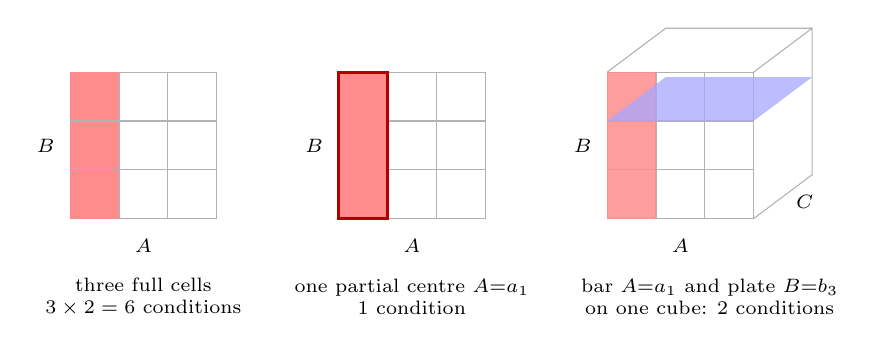
\begin{tikzpicture}[scale=0.62,every node/.style={font=\scriptsize}]
\begin{scope}
\draw[step=1,gray!60] (0,0) grid (3,3);
\fill[red!45] (0,0) rectangle (1,3); \draw[gray!60] (0,1)--(1,1) (0,2)--(1,2);
\node at (1.5,-0.55) {$A$}; \node at (-0.5,1.5) {$B$};
\node[align=center] at (1.5,-1.6) {three full cells\\ $3\times2=6$ conditions};
\end{scope}
\begin{scope}[xshift=5.5cm]
\draw[step=1,gray!60] (0,0) grid (3,3);
\fill[red!45] (0,0) rectangle (1,3); \draw[red!70!black,very thick] (0,0) rectangle (1,3);
\node at (1.5,-0.55) {$A$}; \node at (-0.5,1.5) {$B$};
\node[align=center] at (1.5,-1.6) {one partial centre $A{=}a_1$\\ $1$ condition};
\end{scope}
\begin{scope}[xshift=11cm]
\draw[gray!60] (0,0) grid (3,3);
\draw[gray!60] (3,0)--(4.2,0.9)--(4.2,3.9)--(3,3); \draw[gray!60] (0,3)--(1.2,3.9)--(4.2,3.9);
\fill[red!45,opacity=.85] (0,0) rectangle (1,3);
\fill[blue!35,opacity=.75] (0,2)--(3,2)--(4.2,2.9)--(1.2,2.9)--cycle;
\node at (1.5,-0.55) {$A$}; \node at (-0.5,1.5) {$B$}; \node at (4.05,0.35) {$C$};
\node[align=center] at (2.1,-1.6) {bar $A{=}a_1$ and plate $B{=}b_3$\\ on one cube: $2$ conditions};
\end{scope}
\end{tikzpicture}

\caption{Why fixing every axis costs conditions (schematic; the filled regions are the member cells, which the software draws as a line through them). Left: on the grid of $(A,B)$ the group $A{=}a_1$ is three full cells, six conditions. Middle: the same group as one partial centre, one condition; on the display of $(A,B)$ it is a bar. Right: two groups on different columns of one four-column schema are a bar and a plate of the same cube, two conditions; as full cells of a four-column grid they would be $9+9$ cells at four conditions each.}\label{fig:mech}
\end{figure}

Under a budget of $B$ conditions (Section~\ref{sec:protocol}) the packing becomes budgeted maximum coverage over disjoint candidates; we use the cost-effectiveness greedy with lazy evaluation compared against the best single affordable candidate~\citep{khuller1999}, restricted to candidates disjoint from the chosen ones.

\section{A certificate that survives the search}\label{sec:certificate}

Let $\mathcal{T}$ be the set of distinct row sets among the occupied cells of every partition the search can display: the search partition of every schema with $|S|\le 4$ and, where the capacity rule merged levels, the unmerged partition as well. $T=|\mathcal{T}|$ is fixed once the columns are fixed and does not depend on the target, on $\tau$ or on $m$.

\begin{theorem}[Family-wise certificate]\label{thm:cert}
Conditionally on the columns, let the rows be independent with $\Pr(z_i=1)=p_i$. For a cell $c$ with rows $I_c$ let $\bar p_c=\frac1{n_c}\sum_{i\in I_c}p_i$. Let
\[
k^*(n,\tau,\lambda)=\min\Big\{k:\ k\ge\lceil n\tau\rceil+1,\ \Pr\big(\mathrm{Bin}(n,\tau)\ge k\big)\le\lambda\Big\}.
\]
Then, with $\lambda=\alpha/T$, the probability that some cell $c\in\mathcal{T}$ with $\bar p_c\le\tau$ has $k_c\ge k^*(n_c,\tau,\lambda)$ is at most $\alpha$, simultaneously over every $\tau\in(0,1)$ and every rule by which schemas are chosen after seeing the target.
\end{theorem}

\begin{proof}[Proof sketch]
$k_c$ is Poisson-binomial with mean $n_c\bar p_c$. By Hoeffding's Theorem~4~\citep{hoeffding1956}, for $k-1\ge n\bar p_c$ the upper tail of a Poisson-binomial sum is at most that of $\mathrm{Bin}(n,\bar p_c)$; the threshold is defined as the smallest $k^*$ with (i) $k^*\ge\lceil n\tau\rceil+1$ and (ii) $\Pr[\mathrm{Bin}(n,\tau)\ge k^*]\le\alpha/T$, so that $k^*-1\ge n\tau\ge n\bar p_c$ and the comparison applies. In the implementation (i) is evaluated in exact rational arithmetic and (ii) at the level $\lambda(1-10^{-9})$, so that floating-point rounding of the binomial tail can only withhold a certificate, never grant one. Condition (i) is not cosmetic: without it the binomial test is anti-conservative for heterogeneous rows ($n=3$, $\tau=0.01$, level $0.0298$: the binomial threshold is $k=1$, while rows with $p=(0.03,0,0)$, mean $0.01$, give $\Pr[k\ge1]=0.03$ above the level; by AM--GM the chance of at least one success is smallest when the $p_i$ are equal). Monotonicity of the binomial tail in $p$ gives $\Pr(k_c\ge k^*)\le\Pr(\mathrm{Bin}(n_c,\tau)\ge k^*)\le\alpha/T$ for every cell with $\bar p_c\le\tau$. A union bound over the $T$ cells, which are fixed given the columns, gives the family-wise statement regardless of how the displayed schema was selected. Simultaneity in $\tau$ follows because the event for a larger $\tau$ is contained in that for a smaller one.
\end{proof}

\paragraph{What the theorem does not say.} It bounds the \emph{average} success probability of the rows in a cell, not a population share, and it assumes independence given the columns (families in \texttt{titanic} violate it). The guarantee is per (target value, direction, column set). Westfall--Young resampling was considered and rejected: a permutation of the target tests independence, not $\bar p_c\le\tau$, and certifies a cell of purity $0.85$ as ``$>0.9$''. Tarone's trick removes cells that cannot reach $k^*$ at the given $\tau$ but makes the family depend on $\tau$, which breaks simultaneity for an interactive $\tau$; it is admissible in an experiment with $\tau$ fixed in advance and reduces the smallest certifiable cell only logarithmically: on \texttt{titanic} at $\tau=0.9$ only $K=314$ of the $T=3\,102$ row sets are large enough to reach the threshold at $\alpha/K$, and $n_{\min}$ falls from $105$ to $84$ for a pure cell and from $542$ to $405$ at purity $0.95$ (\texttt{experiments/n\_min\_table.py}; $K$ is the smallest $K$ with at most $K$ testable sets, found by bisection). Columns under Tarone's reduction appear alongside the family bound in Table~\ref{tab:nmin}.

\paragraph{Why not something tighter than a union bound.} The family is the set of distinct row sets, not of descriptions, and that is already the smallest family the display can be held to: two cells with the same rows are one hypothesis, and a cell the search can show but the family omits would be a hypothesis with no error budget. Beyond that, the union bound is the only correction that is valid without an assumption about how the cells depend on each other. The cells of one partition are disjoint, and their counts are independent given the columns, but the cells of different partitions overlap in every way the columns allow --- a 2-D cell contains 3-D cells, two 2-D cells on different column pairs intersect --- and no product-type bound (\v{S}id\'ak, or a step-down over ordered $p$-values that assumes positive dependence) covers arbitrary overlaps of Poisson-binomial sums. What could be gained is bounded: the union bound over $T$ costs $\log T$ in the threshold, and Table~\ref{tab:nmin} shows that from $T=2\,100$ to $T=7\,282\,600$ the smallest certifiable cell grows by a factor of $1.8$; a correction that were exact for the dependence would save part of that factor and nothing of the price of purity, which is where the certificate is expensive.

\paragraph{Price.} Table~\ref{tab:nmin} gives $n_{\min}$, the smallest cell the certificate can certify at $\alpha=0.05$, for a cell all of whose rows carry the target and for a cell whose observed purity is five points above $\tau$, as a function of the family size $T$ (\texttt{experiments/certificate\_price.py}, a standard-library re-implementation of the threshold that reproduces the scipy scan of \texttt{n\_min\_table.py} on every row). From $M=5$ to $M=30$ columns $T$ grows by a factor of $3\,500$ and $n_{\min}$ by $1.8$: the price of the search is logarithmic in the family. The price of purity is not: a five-point margin needs $1\,400$--$2\,600$ rows at $\tau=0.7$ and $500$--$1\,000$ at $\tau=0.9$ whatever $M$, so on tables of a few hundred rows the certificate certifies nothing but pure cells, and at $\tau=0.9$ nothing on \texttt{titanic}. The same table puts the exploratory/holdout split of~\citet{webb2007} beside the family bound: a split tests only the $T_B$ candidates that half~A proposes, but on half the rows, so a cell must be about twice the size in the table that it needs in half~B. On this calculation, with $T_B=10$ candidates, the split needs the same cells as the family bound over $3\,102$ row sets (larger ones for larger $T_B$), and its answer depends on a random division of the rows, which the family bound's does not. The next paragraph shows that on the data the calculation flatters the split.

\begin{table}[t]\centering\footnotesize\setlength{\tabcolsep}{3.5pt}
\caption{Smallest certifiable cell $n_{\min}$ at $\alpha=0.05$, pure / observed purity $\tau+0.05$, for the family certificate ($T$ distinct row sets over $d\le4$ on all rows) and for the exploratory/holdout split with $T_B$ candidates (rows in the whole table, twice the rows half~B needs). Generated by \texttt{experiments/certificate\_price.py}.}\label{tab:nmin}
\begin{tabular}{lrrrrrrr}
\toprule
& & \multicolumn{2}{c}{family} & \multicolumn{2}{c}{family, Tarone} & \multicolumn{2}{c}{split, $T_B=10$}\\
data & $T$ & $\tau=0.7$ & $\tau=0.9$ & $\tau=0.7$ & $\tau=0.9$ & $\tau=0.7$ & $\tau=0.9$\\
\midrule
synthetic ($N=5\,000$, $M=5$) & 2\,100 & 30 / 1365 & 102 / 508 & 28 / 1229 & 85 / 407 & 30 / 1122 & 102 / 444\\
titanic ($N=891$, $M=8$) & 3\,102 & 31 / 1425 & 105 / 542 & 28 / 1229 & 84 / 405 & 30 / 1122 & 102 / 444\\
car\_evaluation ($N=1\,728$, $M=6$) & 3\,391 & 32 / 1437 & 106 / 544 & 28 / 1249 & 79 / 384 & 30 / 1122 & 102 / 444\\
nursery ($N=12\,960$, $M=8$) & 11\,030 & 35 / 1621 & 117 / 606 & 35 / 1621 & 110 / 566 & 30 / 1122 & 102 / 444\\
mushroom ($N=8\,124$, $M=21$) & 49\,254 & 39 / 1853 & 131 / 688 & 38 / 1789 & 122 / 643 & 30 / 1122 & 102 / 444\\
synthetic ($N=5\,000$, $M=10$) & 62\,200 & 40 / 1889 & 134 / 706 & 34 / 1581 & 95 / 467 & 30 / 1122 & 102 / 444\\
chess\_krkp ($N=3\,196$, $M=36$) & 303\,620 & 44 / 2137 & 149 / 803 & 44 / 2105 & 144 / 766 & 30 / 1122 & 102 / 444\\
synthetic ($N=5\,000$, $M=20$) & 1\,316\,400 & 48 / 2365 & 163 / 884 & 40 / 1921 & 106 / 543 & 30 / 1122 & 102 / 444\\
synthetic ($N=5\,000$, $M=30$) & 7\,282\,600 & 53 / 2637 & 179 / 984 & 44 / 2117 & 113 / 584 & 30 / 1122 & 102 / 444\\
\bottomrule
\end{tabular}

\end{table}

\paragraph{Against the holdout split, on the data.} Table~\ref{tab:split} (Appendix~\ref{app:tables}) runs the exploratory/holdout split of~\citet{webb2007} on the same folds as the family certificate (Section~\ref{sec:protocol}: half~A of the training fold proposes under the observed-purity rule, half~B tests every proposed group once at $\alpha/T_B$, $T_B$ the number of distinct groups proposed over the six budgets). The calculation above, which gave the two certificates the same $n_{\min}$ at $T_B=10$, is not what happens: on the ten configurations that certify anything under the family bound, partial centres certified by the split cover less on nine (mean $30$ against $40$ points at $B=32$; \texttt{adult} $3$ against $23$, \texttt{titanic} $0$ against $34$), and on the five that certify nothing under the family bound the split certifies $0$--$4$ points whose held-out purity reaches $\tau$ in at most $12\,\%$ of the splits. Two things the calculation left out account for it. The proposing half sees half the rows, so cells that clear the size floor and the purity rule on the full training fold need not on half of it; and $T_B$ counts every distinct proposal of every budget, not ten. The split is a valid certificate for every method alike, the tree included, and that is its one advantage here; what it certifies are small cells that sit close to $\tau$: the held-out purity of the split-certified union reaches $\tau$ in $49\,\%$ of the splits for partial centres, against $97\,\%$ under the family bound. The family bound tests more hypotheses at a stricter level, but on all the rows, and on these tables that is the better trade.

\paragraph{Power.} Figure~\ref{fig:power} gives the probability that a cell of $n$ rows, each carrying the target with probability $p$, is certified; Table~\ref{tab:n80} the size at which it reaches $0.8$. A pure cell is certified almost surely once it passes $n_{\min}$; a cell at $p=\tau+0.05$ needs roughly $1.4\times n_{\min}$ rows ($2\,020$ at $\tau=0.7$, $729$ at $\tau=0.9$ for the \texttt{titanic} family). In the simulation of \texttt{experiments/certificate\_power.py} (eight 3-level columns, a true centre at purity $0.95$, a cell at exactly $\tau=0.8$, background $0.10$) power under strict control is 1\,\% at $N=500$, 57\,\% at $N=1000$ and 100\,\% at $N=3000$, with a family-wise error of 0 in every setting; the per-schema certificate the product used before has power 0.75 at $N=500$ but a family-wise false-certificate rate of 68\,\% on pure noise at $d\le4$. In the study the certificate is non-empty on 10 of the 19 real configurations (Section~\ref{sec:results}); whether it is worth its price is a question of $N$, $\tau$ and the margin, and Table~\ref{tab:n80} is the answer.

\begin{figure}[t]\centering
% Generated data: fig_certificate_power.dat (experiments/certificate_price.py).
\begin{tikzpicture}
\begin{groupplot}[group style={group size=2 by 1, horizontal sep=14mm},
  width=0.5\linewidth, height=0.36\linewidth, xmode=log, ymin=0, ymax=1.02,
  xmin=10, xmax=3000, xlabel={cell size $n$}, grid=major, grid style={gray!25},
  tick label style={font=\scriptsize}, label style={font=\scriptsize}, title style={font=\small},
  legend style={font=\scriptsize, draw=none, fill=white, fill opacity=0.85, text opacity=1,
                at={(0.03,0.97)}, anchor=north west, cells={anchor=west}}]
\nextgroupplot[title={$\tau=0.7$}, ylabel={$\Pr[\text{certified}]$}]
\addplot[black, thick] table[x=n, y=titanic_t70_p100] {fig_certificate_power.dat};
\addplot[black, thick, dashed] table[x=n, y=chess_t70_p100] {fig_certificate_power.dat};
\addplot[red!70!black, thick] table[x=n, y=titanic_t70_p75] {fig_certificate_power.dat};
\addplot[red!70!black, thick, dashed] table[x=n, y=chess_t70_p75] {fig_certificate_power.dat};
\nextgroupplot[title={$\tau=0.9$}]
\addplot[black, thick] table[x=n, y=titanic_t90_p100] {fig_certificate_power.dat};
\addlegendentry{$p=1$, $T=3\,102$}
\addplot[black, thick, dashed] table[x=n, y=chess_t90_p100] {fig_certificate_power.dat};
\addlegendentry{$p=1$, $T=303\,620$}
\addplot[red!70!black, thick] table[x=n, y=titanic_t90_p95] {fig_certificate_power.dat};
\addlegendentry{$p=\tau+0.05$, $T=3\,102$}
\addplot[red!70!black, thick, dashed] table[x=n, y=chess_t90_p95] {fig_certificate_power.dat};
\addlegendentry{$p=\tau+0.05$, $T=303\,620$}
\end{groupplot}
\end{tikzpicture}

\caption{Probability that a cell of $n$ rows with per-row target probability $p$ is certified at $\alpha=0.05$, for the family sizes of \texttt{titanic} ($T=3\,102$) and \texttt{chess} ($T=303\,620$). Homogeneous rows, the case the threshold is tight for.}\label{fig:power}
\end{figure}

\begin{table}[t]\centering\small
\caption{$n_{80}$: the cell size at which the probability of certification reaches $0.8$, next to $n_{\min}$ (Table~\ref{tab:nmin}).}\label{tab:n80}
\begin{tabular}{llrrrr}
\toprule
$T$ & $\tau$ & $p=\tau+0.05$ & $p=1$ & \multicolumn{2}{l}{$n_{\min}$ (pure / $\tau+0.05$)}\\
\midrule
3\,102 (titanic) & 0.7 & 2020 & 31 & 31 & 1425\\
3\,102 (titanic) & 0.9 & 729 & 105 & 105 & 542\\
303\,620 (chess) & 0.7 & 2856 & 44 & 44 & 2137\\
303\,620 (chess) & 0.9 & 1031 & 149 & 149 & 803\\
\bottomrule
\end{tabular}

\end{table}

\section{Evaluation protocol}\label{sec:protocol}

\paragraph{Folds.} Repeated stratified $K$-fold ($5\times5$; $5\times2$ for \texttt{mushroom} and \texttt{adult}, $5\times1$ for \texttt{chess}, \texttt{connect\_4} and \texttt{splice}, where one repeat is what the budget allowed), identical across methods so that differences are paired. On the three single-repeat tables the Nadeau--Bengio $t$ has four degrees of freedom, so a mark there is weaker evidence than elsewhere; the $p$-values behind the Holm columns of Table~\ref{tab:counts} use the degrees of freedom of each table. Every fitted quantity --- bins are fixed, but the capacity rule, level merging and the family size $T$ --- is computed on the training fold; the chosen groups are carried to the held-out rows through the fitted partition (unseen levels go to the ``other'' group).

\paragraph{Budget.} All methods answer the same question: with at most $B\in\{1,2,4,8,16,32\}$ conditions, which groups of rows hold the most positives, each at training purity $\ge\tau$ (or certified by the family bound, or proposed on half of the training fold and certified on the other half) and size $\ge m$? A cell of a $d$-column grid costs $d$; a rule of length $\ell$ costs $\ell$; a tree leaf costs its depth.

\paragraph{Methods.}
\texttt{vsf}: best schema per budget, its top $\lfloor B/d\rfloor$ centres.
\texttt{vsf\_partial}: best schema per budget with partial centres, disjoint greedy.
\texttt{vsf\_greedy}: the nested chain $S_1\subset S_2\subset S_3\subset S_4$ (the greedy the exhaustive search argues against).
\texttt{rules}: every conjunction of $\le 4$ conditions occurring in the training rows, budgeted maximum coverage (may overlap).
\texttt{rules\_pure}: \texttt{rules} with the union kept at training purity $\ge\tau$.
\texttt{rules\_disjoint}: \texttt{rules} with no shared training row.
\texttt{tree}: CART on one-hot columns, best over depth $\le 4$, criterion and class weight; qualifying leaves under the same greedy. Under the certified rule the tree's leaves are not a pre-specified family, so the filter is only a filter, not a certificate (see below).
\texttt{wracc}: the qualifying family of \texttt{rules} ranked by weighted relative accuracy $\mathrm{WRAcc}=\frac{n}{N}\big(\frac{k}{n}-\frac{P}{N}\big)$, the default quality of subgroup discovery (pysubgroup, SD-Map, CN2-SD), read as a top-$k$ list: rules taken in that order while they fit the budget, overlaps allowed. What ``a subgroup-discovery tool with a purity filter'' returns.
\texttt{wracc\_raw}: the same list without the purity filter (size $\ge m$ only, the 256 best cells by WRAcc): what the tool returns out of the box. Not a solution of the task, kept to show what the purity floor changes.
\texttt{tree\_opt}: an optimal tree (DL8.5,~\citealp{aglin2020}; package \texttt{pydl8.5}) of depth $\le d$ for each $d\le4$ on one-hot columns, minimising the class-weighted error with weights $1:\tau/(1-\tau)$, whose optimum over leaves is net coverage; the weights are realised by replicating rows (for $\tau=0.7$ positives three times, negatives seven), so the search is exact and needs no callback. Leaves are then treated exactly as CART's. Run on 14 of the 17 tables: not on \texttt{adult} and \texttt{connect\_4}, where the replicated one-hot matrix has $2$--$4\times10^5$ rows and a depth-4 fit exceeds the time budget. No fit on the other tables hit the ten-minute limit.
\texttt{ssdpp}: SSD++~\citep{proenca2022}, an MDL rule list fitted on the training fold for the two-class target (beam 50, depth $\le4$, minimum support $m$); a rule list is ordered, so its $i$-th rule applies to the rows no earlier rule matched and its groups are disjoint by construction. Its qualifying rules enter the same budgeted greedy at cost = conditions. This is the strongest published subgroup-set method with a redundancy control; its objective (compression of the whole target column) differs from ours, and the list also holds rules for the other class, which never qualify. The package's PyPI release needs a compatibility patch for current numpy/pandas that we ship and apply deterministically.

\paragraph{Certified selection for the baselines.} Under the certified rule every method qualifies a group by the same threshold $k^*(n,\tau,\alpha/T)$, with $T$ the family of Section~\ref{sec:certificate} computed on the training fold. For \texttt{rules}, \texttt{rules\_pure} and \texttt{rules\_disjoint} this is a valid post-selection certificate, not merely the same filter: a conjunction of $\ell\le4$ conditions on the columns $S$ that occurs in the training rows is an occupied cell of the partition of $S$ (of the unmerged partition where the capacity rule merged levels), so its row set is a member of $\mathcal{T}$, and the candidate family of the rules baseline is the family of the grid search. The same holds for \texttt{vsf\_greedy}. For the tree and for SSD++ it is only a filter: a leaf is grown on the target, and the $i$-th rule of a list applies to the residue of the first $i-1$, which is not a cell of any partition.

\paragraph{Metrics.} On the held-out rows: coverage $k/P$ of the union of selected groups; purity $k/n$ of the union; net coverage $(k-\frac{\tau}{1-\tau}(n-k))/P$, the Lagrangian of coverage subject to purity $\ge\tau$; share of splits with held-out purity $\ge\tau$; description stability (mean pairwise Jaccard of the selected row sets across splits); conditions actually spent; selection time. Paired differences with the Nadeau--Bengio corrected variance~\citep{nadeau2003}; a mark needs $|t|\ge 2$, and Table~\ref{tab:counts} also reports the marks that survive a Holm correction over the budgets of each configuration. Wins and losses are counted over (configuration, budget) cells and read as descriptive counts: the six budgets of one configuration share the same splits and are not independent, and the correction does not span configurations.

\paragraph{Why the disjoint baseline.} Under the observed-purity rule the held-out purity of the \texttt{rules} union reaches $\tau$ in 60\,\% of the splits, against 77--79\,\% for \texttt{vsf}, \texttt{vsf\_partial} and \texttt{rules\_disjoint} (Table~\ref{tab:counts}; the independent re-implementation of Section~\ref{sec:results} gave 53 against 73\,\%). Each rule is at purity $\ge\tau$ on the training rows; their union is not, because the rules overlap on the rows that carry the target and not on the others. A comparison of coverage alone between an overlapping and a disjoint method therefore compares different constraints.

\section{Data}\label{sec:data}
Seventeen real tables with pinned SHA-256 hashes and recorded preprocessing (Table~\ref{tab:data}), and two planted designs. The real tables are the UCI classics of subgroup discovery (\texttt{mushroom}, \texttt{nursery}, \texttt{car}, \texttt{chess}), \texttt{titanic}, three small clinical tables, two wide PMLB tables (\texttt{connect\_4}, $67\,557\times42$; \texttt{splice}, $3\,188\times60$, where every method is capped at $d\le3$ because the size-4 families are too large for all of them alike), seven tables from public mirrors with $N$ from 1\,470 to 48\,842 and base rates from 8 to 28\,\% (\texttt{adult}, \texttt{hmda}, \texttt{credit}, \texttt{resume}, and three vendor tables that are synthetic or demonstration data rather than observations: IBM's fictional \texttt{attrition}, IBM's \texttt{wa\_churn} demo and the \texttt{mlc\_churn} table the C5.0 package describes as artificial). \texttt{car}, \texttt{nursery} (full factorial designs from a decision model), \texttt{chess} and \texttt{connect\_4} (endgame enumerations) and \texttt{mushroom} (hypothetical specimens from a field guide) are deterministic or generated; the observational tables are \texttt{adult}, \texttt{hmda}, \texttt{credit}, \texttt{resume}, \texttt{titanic}, \texttt{splice} and the three clinical tables. Of the ten configurations that certify anything, only \texttt{adult}, \texttt{hmda} and \texttt{titanic} are observational. The planted designs are \emph{aligned} (one 4-cell and one 2-cell in the same four columns) and \emph{misaligned} (two 2-condition rules on disjoint column pairs, which no full grid of four columns can show with fewer than $9+9$ cells). Three high-dimensional expression tables (325--7\,070 columns) are in the repository but excluded: exhaustive search over $d\le4$ needs a feature pre-filter, which would enter the family and break Theorem~\ref{thm:cert}.

\begin{table}[t]\centering\small
\caption{Datasets and settings (generated by \texttt{experiments/paper\_tables.py} from the manifest and the configuration list).}\label{tab:data}
\begin{tabular}{lrrlrrl}
\toprule
dataset & $N$ & $M$ & positive value & base rate & $\tau/\text{base}$ & $\tau$ / $m$ / repeats\\
\midrule
titanic & 891 & 8 & survived & 38\,\% & 1.8 & 0.7/1/5; 0.9/1/5; 0.9/20/5\\
breast\_cancer & 286 & 9 & recurrence-events & 30\,\% & 2.4 & 0.7/1/5\\
thyroid\_recurrence & 383 & 16 & Yes & 28\,\% & 3.2 & 0.9/1/5\\
breast\_cancer\_wisconsin & 699 & 9 & malignant & 34\,\% & 2.6 & 0.9/1/5\\
car\_evaluation & 1728 & 6 & acc & 22\,\% & 4.1 & 0.9/1/5\\
nursery & 12960 & 8 & spec\_prior & 31\,\% & 2.9 & 0.9/1/5\\
nursery & 12960 & 8 & priority & 33\,\% & 2.1 & 0.7/1/5\\
mushroom & 8124 & 21 & poisonous & 48\,\% & 1.9 & 0.9/1/2\\
chess\_krkp & 3196 & 36 & won & 52\,\% & 1.7 & 0.9/1/3\\
adult & 48842 & 12 & \textgreater{}50K & 24\,\% & 2.9 & 0.7/20/2\\
hmda & 2380 & 12 & yes & 12\,\% & 4.2 & 0.5/20/5\\
attrition & 1470 & 19 & Yes & 16\,\% & 3.1 & 0.5/20/5\\
credit & 4454 & 13 & bad & 28\,\% & 2.5 & 0.7/20/5\\
resume & 4870 & 24 & yes & 8\,\% & 3.7 & 0.3/20/5\\
wa\_churn & 7043 & 19 & Yes & 27\,\% & 2.6 & 0.7/20/5\\
mlc\_churn & 5000 & 11 & yes & 14\,\% & 5.0 & 0.7/20/5\\
connect\_4 & 67557 & 42 & loss & 25\,\% & 2.8 & 0.7/20/1\\
connect\_4 & 67557 & 42 & win & 66\,\% & 1.4 & 0.9/20/1\\
splice & 3188 & 60 & site\_b & 24\,\% & 3.7 & 0.9/20/3\\
\bottomrule
\end{tabular}

\end{table}

\section{Results}\label{sec:results}

\subsection{The price of one grid, and where it comes from}\label{sec:mechanism}

\begin{table}[t]\centering\small
\caption{Paired comparisons over (configuration, budget) cells; uninformative cells (no method above 1\,\% held-out coverage) left out. Left: the descriptive mark, $|t|\ge2$ on the Nadeau--Bengio $t$ with $J-1$ degrees of freedom ($J$ splits; a two-sided level of about $0.06$ at $5\times5$ and $0.12$ at $5\times1$). Right: cells whose two-sided $p$-value survives a Holm correction over the informative budgets of the same configuration at $0.05$. Neither correction spans configurations: these are counts of cells, not a test of one global hypothesis. The \emph{split} block is the holdout certificate of Section~\ref{sec:certificate}. ``Gap closed'' is $(\cov^{\mathrm{p}}-\cov)/(\cov_{\mathrm{rules\,disj}}-\cov)$ over cells where disjoint rules beat the grid by at least one point.}\label{tab:counts}
\begin{tabular}{llrrrrrr}
\toprule
& & \multicolumn{3}{c}{$|t|\ge2$} & \multicolumn{3}{c}{Holm within configuration}\\
selection & comparison & better & tie & worse & better & tie & worse\\
\midrule
certified & full grid vs disjoint rules & 2 & 31 & 20 & 2 & 35 & 16\\
certified & partial centres vs disjoint rules & 2 & 45 & 6 & 2 & 48 & 3\\
certified & partial centres vs full grid & 18 & 35 & 0 & 12 & 41 & 0\\
certified & \multicolumn{7}{l}{gap closed by partial centres: median 1.00, mean 0.86 ($n=21$)}\\
certified & \multicolumn{7}{l}{held-out union purity $\ge\tau$: grid 97\,\%, partial 97\,\%, rules$_{\mathrm{disj}}$ 97\,\%, rules 97\,\%}\\
\midrule
purity & full grid vs disjoint rules & 2 & 62 & 45 & 1 & 66 & 42\\
purity & partial centres vs disjoint rules & 5 & 83 & 21 & 2 & 91 & 16\\
purity & partial centres vs full grid & 41 & 68 & 0 & 39 & 70 & 0\\
purity & \multicolumn{7}{l}{gap closed by partial centres: median 0.85, mean 0.75 ($n=55$)}\\
purity & \multicolumn{7}{l}{held-out union purity $\ge\tau$: grid 79\,\%, partial 79\,\%, rules$_{\mathrm{disj}}$ 77\,\%, rules 60\,\%}\\
\bottomrule
\end{tabular}

\end{table}

\begin{table}[t]\centering\small
\caption{Held-out coverage (\%) at $B=32$, observed-purity selection. Marks: partial centres vs the full grid (p\,vs\,g) and vs disjoint rules (p\,vs\,r).}\label{tab:purity32}
\begin{tabular}{llrrrrrcc}
\toprule
dataset & $\tau$ & grid & partial & rules$_{\mathrm{disj}}$ & rules & tree & p$\,$vs$\,$g & p$\,$vs$\,$r\\
\midrule
titanic & 0.9 & 48 & 53 & 57 & 59 & 51 & + & -\\
titanic & 0.7 & 67 & 73 & 77 & 85 & 70 & + & -\\
titanic ($m{=}20$) & 0.9 & 47 & 46 & 47 & 53 & 47 & = & =\\
breast\_cancer & 0.7 & 27 & 32 & 39 & 49 & 30 & = & =\\
thyroid\_recurrence & 0.9 & 83 & 88 & 88 & 89 & 85 & = & =\\
breast\_cancer\_wisconsin & 0.9 & 82 & 85 & 75 & 94 & 89 & = & +\\
car\_evaluation & 0.9 & 21 & 21 & 12 & 12 & 0 & = & +\\
nursery (spec\_prior) & 0.9 & 42 & 57 & 59 & 68 & 28 & + & -\\
nursery (priority) & 0.7 & 63 & 86 & 87 & 90 & 67 & + & -\\
mushroom & 0.9 & 99 & 100 & 100 & 100 & 100 & + & =\\
chess\_krkp & 0.9 & 84 & 84 & 92 & 98 & 41 & = & -\\
adult & 0.7 & 31 & 42 & 44 & 63 & 20 & + & =\\
hmda & 0.5 & 19 & 29 & 27 & 51 & 30 & + & =\\
attrition & 0.5 & 34 & 43 & 47 & 69 & 34 & + & -\\
credit & 0.7 & 17 & 24 & 30 & 50 & 17 & + & -\\
resume & 0.3 & 4 & 4 & 15 & 18 & 4 & = & -\\
wa\_churn & 0.7 & 30 & 33 & 37 & 49 & 30 & + & -\\
mlc\_churn & 0.7 & 16 & 25 & 33 & 50 & 21 & + & -\\
connect\_4 (loss) & 0.7 & 10 & 10 & 19 & 27 & 11 & + & -\\
connect\_4 (win) & 0.9 & 27 & 30 & 39 & 55 & 11 & + & -\\
splice & 0.9 & 4 & 4 & 4 & 5 & 0 & = & =\\
\bottomrule
\end{tabular}

\end{table}

\begin{table}[t]\centering\small
\caption{Held-out coverage (\%) at $B=32$, certified selection (configurations where some method certifies anything).}\label{tab:cert32}
\begin{tabular}{llrrrrrcc}
\toprule
dataset & $\tau$ & grid & partial & rules$_{\mathrm{disj}}$ & rules & tree & p$\,$vs$\,$g & p$\,$vs$\,$r\\
\midrule
titanic & 0.7 & 34 & 34 & 34 & 35 & 52 & = & =\\
nursery & 0.9 & 42 & 49 & 49 & 58 & 23 & + & =\\
nursery & 0.7 & 40 & 61 & 67 & 68 & 67 & + & -\\
mushroom & 0.9 & 96 & 98 & 98 & 100 & 96 & + & =\\
chess\_krkp & 0.9 & 57 & 81 & 81 & 94 & 41 & + & =\\
adult & 0.7 & 16 & 23 & 22 & 42 & 14 & + & =\\
hmda & 0.5 & 15 & 15 & 15 & 15 & 15 & = & =\\
mlc\_churn & 0.7 & 9 & 9 & 9 & 9 & 12 & = & =\\
connect\_4 & 0.7 & 6 & 6 & 12 & 17 & 10 & = & -\\
connect\_4 & 0.9 & 19 & 27 & 34 & 43 & 11 & + & -\\
\bottomrule
\end{tabular}

\end{table}

\begin{figure}[t]\centering
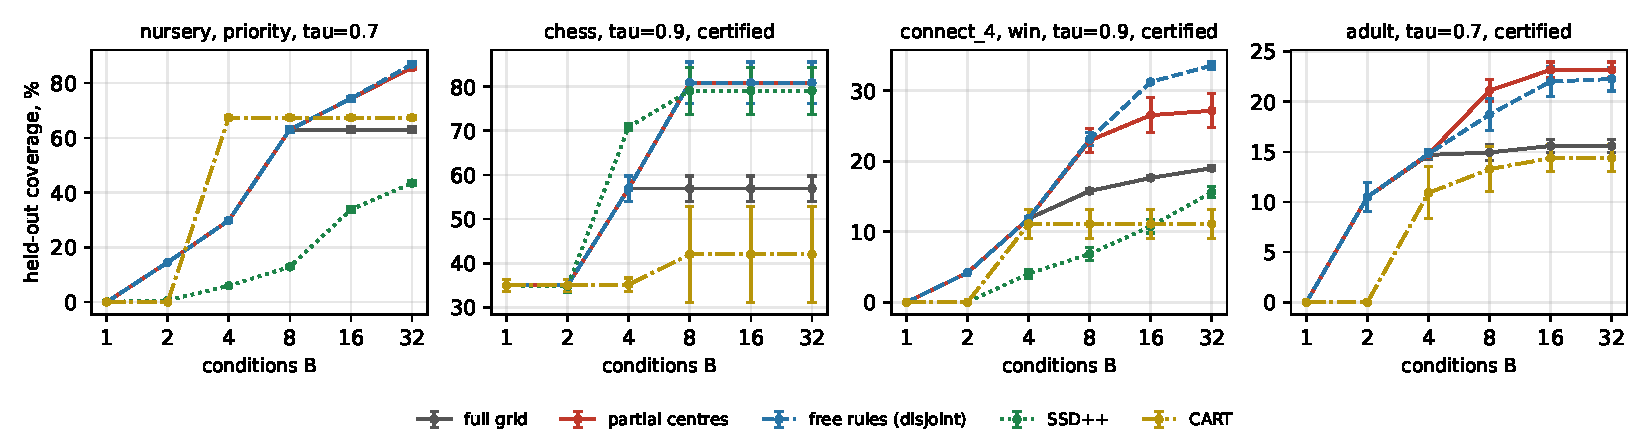
\includegraphics[width=\linewidth]{fig_coverage_budget}
\caption{Held-out coverage against the condition budget on four tables (mean $\pm$ Nadeau--Bengio SE over splits). Partial centres follow free disjoint rules where the full grid stalls; \texttt{connect\_4} is the table where one schema cannot hold what forty-two columns offer.}\label{fig:budget}
\end{figure}

Table~\ref{tab:counts} gives the counts over the 21 observed-purity and 10 certified configurations that are informative (some method above 1\,\% held-out coverage); Figure~\ref{fig:budget} shows four of them against the budget. With the observed-purity rule the full grid loses to free disjoint rules in 45 of 109 cells and wins 2; with partial centres the same schema family loses 21 and wins 5, and closes a median 85\,\% of the gap. Under the certificate the full grid loses 20 of 53 cells; partial centres lose 6 (all on \texttt{connect\_4}, Section~\ref{sec:ssdpp}) and win 2. The Holm columns of Table~\ref{tab:counts} thin the marks without moving the picture: partial centres still lose 16 observed-purity cells and 3 certified ones to disjoint rules, and still never lose to the full grid (39 and 12 wins survive). The observed-rule losses are at $B\ge16$ (20 of 21) on the tables with the most columns to spare (\texttt{connect\_4}, \texttt{mlc\_churn}, \texttt{credit}, \texttt{attrition}, \texttt{resume}, \texttt{wa\_churn}: Table~\ref{tab:purity32}), where free rules keep adding disjoint fragments from other columns after the schema's four are exhausted.

On the misaligned design the full grid covers 0.375 at every budget (one rule; the second needs nine 4-condition cells) while partial centres reach 0.718 at $B=16$, equal to free rules; on the aligned design the full grid still loses (0.504 vs 0.544) because the planted 2-cell costs nine full cells. At $B=32$ the full grid spends on average 7 conditions: one grid holds few pure fully specified cells. This is the mechanism of Figure~\ref{fig:mech}: the alignment price is the price of fixing every axis.

\subsection{Compactness of the description}\label{sec:compact}
\begin{table}[t]\centering\small
\caption{Compactness at $B=32$ over the informative configurations on which every method ran (\texttt{experiments/compactness.py}). Coverage and conditions spent are held-out means over all splits; groups and distinct columns named by the description are counted on the first split, since the column set is not recorded per split. The tree and SSD++ record no column labels.}\label{tab:compact}
\begin{tabular}{llrrrrr}
\toprule
selection & method & cells & coverage & conditions & groups & columns\\
\midrule
purity & full grid & 21 & 0.41 & 17.3 & 5.1 & 3.0\\
purity & partial centres & 21 & 0.46 & 16.4 & 5.5 & 3.9\\
purity & greedy chain & 21 & 0.35 & 13.5 & 4.6 & 2.6\\
purity & rules$_{\mathrm{disj}}$ & 21 & 0.49 & 22.3 & 7.6 & 8.3\\
purity & rules & 21 & 0.59 & 26.6 & 10.1 & 10.2\\
purity & tree & 21 & 0.37 & 7.7 & 2.7 & --\\
purity & SSD++ & 21 & 0.39 & 14.8 & 5.2 & --\\
\midrule
certified & full grid & 10 & 0.33 & 7.7 & 2.9 & 2.6\\
certified & partial centres & 10 & 0.40 & 8.8 & 3.5 & 3.3\\
certified & greedy chain & 10 & 0.30 & 6.8 & 3.0 & 2.2\\
certified & rules$_{\mathrm{disj}}$ & 10 & 0.42 & 11.7 & 4.0 & 4.4\\
certified & rules & 10 & 0.48 & 18.5 & 6.7 & 7.1\\
certified & tree & 10 & 0.34 & 3.9 & 1.4 & --\\
certified & SSD++ & 10 & 0.32 & 14.8 & 4.5 & --\\
\bottomrule
\end{tabular}

\end{table}

A budget of conditions bounds the length of the description; Table~\ref{tab:compact} reports what the methods actually spend at $B=32$ and how many columns the reader has to hold. Under the observed-purity rule partial centres reach 94\,\% of the coverage of free disjoint rules ($0.46$ against $0.49$) with 74\,\% of the conditions ($16.4$ against $22.3$) and fewer than half the columns ($3.9$ against $8.3$); overlapping rules reach $0.58$ by naming ten columns and spending $26$ conditions on groups whose union does not hold $\tau$ (Table~\ref{tab:counts}). Under the certificate the pattern is the same ($0.40$ against $0.42$ coverage, $8.8$ against $11.7$ conditions, $3.3$ against $4.4$ columns). The full grid and the trees (Section~\ref{sec:treeopt}) are more compact still; the full grid and CART cover less for it, the optimal tree does not; the greedy chain is compact because it stops early. The column count of a grid method is bounded by four by construction; that of free rules grows with the budget, since every further disjoint fragment may come from a new column. Together with the certificate, this is the measurable part of what the one-grid constraint buys over free rules.

\subsection{Under the certificate}
Table~\ref{tab:cert32}. Of the 19 certified configurations on real tables, 10 certify anything at all; the nine that do not are the three clinical tables ($N\le700$), \texttt{car}, \texttt{credit}, \texttt{resume}, \texttt{wa\_churn}, \texttt{attrition} and \texttt{splice}, where no cell reaches $n_{\min}$ at its $\tau$ (Section~\ref{sec:certificate}). Of the six planted designs, the three at $N=2\,000$ certify next to nothing (\emph{xor} 7.5\,\%, the other two 0) and the three at $N=20\,000$ certify 90--96\,\% of the positives. The paired counts below are over the ten informative real configurations (53 cells). Where something is certified, one schema with partial centres ties free disjoint rules in 45 of 53 cells, wins 2 (\texttt{mushroom} at $B\le4$) and loses 6, all on \texttt{connect\_4}; against the full grid it is never worse and better in 18 of 53 cells; an independent re-implementation of the three candidate families without the \texttt{vsf} package (\texttt{experiments/partial\_centres\_external.py}: no capacity rule, no level merging, $5\times3$ folds), run on \texttt{titanic}, \texttt{adult}, \texttt{hmda}, \texttt{credit}, \texttt{wa\_churn}, \texttt{mlc\_churn} and the two planted designs before those tables entered the study, gave 77 ties, 2 wins, 0 losses over 79 cells: the mechanism does not depend on the implementation. Held-out union purity reaches $\tau$ in 97\,\% of splits for every method under the certificate, against 60\,\% for overlapping rules under the observed rule (Table~\ref{tab:counts}).

\subsection{Net coverage and stability}\label{sec:net}

Coverage alone rewards a method that adds fragments whose purity does not hold up, so Table~\ref{tab:net32} (Appendix~\ref{app:tables}) puts the two numbers side by side for every configuration. Net coverage, $(k - \tfrac{\tau}{1-\tau}(n-k))/P$ over the held-out union, is the Lagrangian of ``cover the most target rows subject to purity $\ge\tau$'': a group at purity exactly $\tau$ adds nothing, a union below $\tau$ scores negative. The ordering differs between the two selection rules. Under the certificate, mean net coverage over the informative cells is $0.23$ for partial centres, $0.23$ for the full grid, $0.22$ for disjoint and for overlapping rules and $0.19$ for the tree (SSD++ and the optimal tree are ahead of all of these; Sections~\ref{sec:treeopt} and~\ref{sec:ssdpp}). Under the observed-purity rule it is $0.16$ for the full grid and for partial centres, $0.13$ for disjoint rules and the tree and $0.05$ for overlapping rules; on net coverage partial centres beat overlapping rules in 44 of 109 cells and lose 2: the freer the description, the more of its training coverage is fragments that do not survive the held-out fold (\texttt{titanic}, $\tau=0.7$: overlapping rules $-0.24$, disjoint rules $0.07$, partial centres $0.08$, full grid $0.15$). With $m=20$ the three disjoint methods are within a few points of each other on every table. The lesson is a selection-discipline effect, not a grid effect: the full grid's cells are large because they are few, and a size floor gives the freer methods the same protection.

Description stability (mean pairwise Jaccard of the selected rows across splits) does not separate the methods: medians $0.82$--$0.92$ under both rules, the tree highest ($0.90$--$0.92$) and partial centres and disjoint rules lowest ($0.82$--$0.87$). A freer description is chosen from more candidates and varies more between samples; the difference is small.

\subsection{Trees and greedy chains}\label{sec:trees}
A depth-$\le4$ CART tree with $\min\_samples\_leaf=m$, the best over criterion and class weight at each budget, is the natural competitor that also names at most four columns per leaf and partitions the rows. Under the observed-purity rule partial centres beat it (paired $|t|\ge2$) in 39 of 109 cells and lose 10 (at $B=32$: 9 wins, 12 ties, no loss); under the certificate 22 / 17 / 14 (at $B=32$: 5 / 3 / 2), but the tree's filter is not a certificate: its leaves are grown on the target, not drawn from a family fixed before the target is read, so the 51.7 vs 34.2 it scores on \texttt{titanic} at $\tau=0.7$ carries no guarantee: its held-out union purity there is $0.89$ against $0.95$ for the certified grid, the leaves the filter passed being ones a certificate over a fixed family would not. On the planted grid design CART is greedy at the root and covers 2--4\,\% (\texttt{experiments/compare\_baselines.py --synthetic grid}). Section~\ref{sec:treeopt} runs the optimal tree.

The greedy schema chain $S_1\subset S_2\subset S_3\subset S_4$ (add the column that most improves the ranking key) is worse than the exhaustive winner in 33 of 109 cells under the observed rule and 9 of 53 under the certificate, never better (mean gap at $B=32$: 6.2 and 3.4 points); on \texttt{chess} it never leaves the 1D winner (35\,\% against 84\,\% and 57\,\% exhaustive). This is the synergy case the exhaustive search exists for.

\subsection{Optimal trees}\label{sec:treeopt}

The optimal tree is the strongest single-partition competitor in the study, and the comparison is not one-sided (Table~\ref{tab:treeopt}, Appendix~\ref{app:tables}). On held-out coverage under the observed-purity rule partial centres beat it in 27 of 93 cells and lose 12 (at $B=32$: $0.49$ against $0.47$ mean coverage); under the certificate they win 8 and lose 10 ($0.50$ against $0.51$). On net coverage the optimal tree is clearly ahead under both rules ($0.22$ against $0.15$ and $0.43$ against $0.36$ at $B=32$): it optimises exactly that quantity, and its leaves are few and large. Where it loses coverage it loses it for the reason CART does, one partition of the rows: on \texttt{attrition}, \texttt{credit} and \texttt{wa\_churn} partial centres cover $5$--$12$ points more, on \texttt{chess} and \texttt{mlc\_churn} the tree covers $5$--$13$ more. Two caveats keep this from being the last word. The tree's leaves are grown on the target, so under the certified rule the threshold is a filter and not a certificate, exactly as for CART; and the two widest tables, where the one-grid constraint costs most, are the two the solver did not run on. What the comparison settles is narrower and worth stating: the CART numbers of Section~\ref{sec:trees} are not an artefact of a greedy tree. Against the coverage-tuned CART the optimal weighted tree covers more on six tables at $B=32$ and less on six; optimality buys net coverage, not coverage.

\subsection{WRAcc lists}\label{sec:wracc}
A WRAcc-ranked list is what a subgroup-discovery tool returns, and the purity floor is what our task adds to it. With the floor applied the list is the family of free rules in a different order, and the order costs coverage against budgeted maximum coverage over the same rules ($0.49$ against $0.60$ at $B=32$ under the observed rule) while it gains held-out purity (the union reaches $\tau$ in $68\,\%$ of the splits against $58\,\%$ for maximum coverage): the top of a WRAcc ranking is the large, clean rules. Against partial centres it is a near tie in coverage ($0.49$ against $0.49$; partial centres win 22 of 99 cells and lose 7, under the certificate 10 and 1) with lower held-out purity ($68$ against $77\,\%$ of splits). Without the floor the list is not a solution of the task at all: it covers far more ($0.87$ at $B=32$, beating partial centres in 75 of 99 cells) with a union that reaches $\tau$ in $18\,\%$ of the splits, and in none of them on 16 of the 19 configurations at $B=32$ (\texttt{sex = female} first on \texttt{titanic}, purity $0.73$, then rules that add rows faster than positives). The purity floor, not the search, is what separates a description of where the target lives from a ranking of where it is over-represented; a tool run out of the box answers the second question. \texttt{connect\_4} is not in these counts (the rule enumeration on $54\,000$ rows and 42 columns was not repeated for the two lists).

\subsection{SSD++}\label{sec:ssdpp}
SSD++ optimises compression of the whole target column, not coverage at a purity floor, and the comparison shows both sides of that. On held-out coverage at $\tau$ partial centres beat it in 63 of 109 observed-purity cells and lose 15 (certified: 34 / 16 / 3); at $B=32$ its mean coverage is $0.39$ against $0.46$ (certified $0.32$ against $0.40$). On held-out purity it is the highest of the methods run on every table: $0.96$ under the certificate and $0.83$ under the observed rule against $0.91$ and $0.76$ for partial centres, and among those methods its net coverage at $B=32$ is highest under both rules ($0.31$ and $0.26$ against $0.28$ and $0.14$ for partial centres); the optimal tree, run on 14 tables, is higher still on its cells (Section~\ref{sec:treeopt}). The two facts are the same fact, and Table~\ref{tab:net32} shows them per configuration: a rule list stops adding rules when they no longer pay for themselves in code length, so what it returns is small and clean; a coverage objective keeps adding groups at exactly $\tau$, and every such group lowers the net score. We do not claim that partial centres beat SSD++; on the objective SSD++ optimises they do not. The paper's task fixes the objective at coverage under a purity floor, and on that objective one grid with partial centres is ahead; a reader whose question is ``the cleanest small description'' should prefer the rule list. One more property of the list matters for the comparison: its $i$-th rule applies to the residue of the first $i-1$, including rules for the \emph{other} class, so a later rule can be pure on the residue where no conjunction is pure on the table. On \texttt{splice} ($\tau=0.9$, $m=20$) every conjunctive family of length $\le3$ is empty on every training fold, all grid and rule methods cover $0.4\,\%$, and SSD++ covers $20\,\%$ at held-out purity $0.81$, below $\tau$. Ordered ``else'' semantics is a description language of its own; partial centres could adopt it (a plate minus an earlier bar is still a region of the same cube) and we leave that as future work.

\paragraph{Where the grid still costs: \texttt{connect\_4}.} All six certified losses to disjoint rules are on \texttt{connect\_4} ($67\,557\times42$, three values per cell): at $\tau=0.9$, $B=32$, partial centres cover $27\,\%$ against $34\,\%$ for disjoint rules ($43\,\%$ overlapping); at $\tau=0.7$, $6\,\%$ against $12\,\%$. Free rules choose their four columns per rule and forty-two columns give them many pure four-cell conjunctions on different boards; one schema cannot hold them. This is the case the one-grid constraint was expected to lose, and it does; on \texttt{chess} ($M=36$) partial centres and disjoint rules tie at $81\,\%$ where the full grid has $57\,\%$.

\subsection{Ablations: capacity rule and size floor}\label{sec:ablation}
\texttt{experiments/ablations.py} varies the capacity divisor ($N_{\mathrm{train}}/5$, $/10$, $/20$, no merging) and the size floor $m\in\{1,5,20\}$ on eight tables at $B=32$. The capacity rule is inert on seven of them: the winning schemas never reach the ceiling, and coverage changes by at most $0.1$ points. On \texttt{car\_evaluation}, a full factorial design of $1\,728$ rows at the ceiling, every change loses coverage --- $-7.1$ points with a looser rule ($N/5$) or none, $-8.6$ with a tighter one ($N/20$) --- for the full grid and for partial centres alike: merged levels pool sparse cells above the floor, and merging further splits the target. The rule is therefore not a tuning knob that favours the method; it is a display constraint that costs nothing on most tables and a few points on one.

The size floor is the lever that matters, and it acts on the freer descriptions most. From $m=1$ to $m=20$ disjoint rules lose $4.6$ points of coverage and raise the share of splits whose held-out purity reaches $\tau$ from $77$ to $91\,\%$; partial centres lose $3.7$ points ($85\to87\,\%$); the full grid loses $3.0$ ($94\to83\,\%$: its cells being large already, the floor removes the few small pure ones it had). Conditions spent at $B=32$ fall from $29$ to $14$ for rules and from $25$ to $13$ for partial centres. Section~\ref{sec:net} is the same effect seen through net coverage.

\subsection{Cost}
Selection time per split (mean over budgets and selection rules, one core): full grid 7.3\,s and partial centres 8.4\,s on \texttt{adult} ($N=48\,842$, $M=12$); 5.9 / 9.8\,s on \texttt{chess} ($N=3\,196$, $M=36$, $58\,905$ schemas of size~4); 2.2 / 9.6\,s on \texttt{mushroom}; under one second on every table with $M\le 20$ and $N\le 8\,000$. The partial search enumerates no new cells; its extra cost is the disjoint packing over the pool of each schema, which grows with the number of qualifying sub-cells (\texttt{mushroom}, $\tau=0.9$, has many). Free rules cost the same as the grid on every table; the tree is fastest. SSD++ is the outlier: on \texttt{adult} its fit took between 80\,s and 15\,h per split under the certified selection (median under two minutes), the MDL beam search occasionally running out to the 40-rule cap; the other methods vary by a factor of two at most across splits.

\section{Conclusion}
The one-grid constraint was measured, not assumed, and what it buys is narrower than the display it came from suggests but real. It buys a certificate: the cells of every grid of at most four columns are a family fixed before the target is read, and a union bound over the $T$ distinct row sets of that family, with a threshold valid for heterogeneous rows, certifies a cell whatever rule chose its grid and simultaneously for every $\tau$. The price is computed exactly, is logarithmic in the number of columns and heavy in purity, and is empty on tables of a few hundred rows; on the same folds it beats the holdout split, the one alternative that applies to every method, by a quarter of the certified coverage and by the share of certified unions that hold $\tau$ on held-out rows (97 against 49\,\%). No tree has such a family. The constraint's cost is coverage, and the cost is the requirement to fix every axis, not to share the columns: partial-axis centres remove it on every table but the widest (\texttt{connect\_4}, where one schema of four columns cannot hold what forty-two columns offer to free rules), and under the certificate they are level with free disjoint rules and with an optimal depth-4 tree fitted to the same objective, at fewer conditions and fewer than half the columns of the free rules. The optimal tree is ahead on net coverage and more compact, and a reader who does not need the certificate should prefer it. The comparison also fixed two things about how such methods should be compared: an overlapping union of rules each at purity $\tau$ is not at purity $\tau$, and a size floor is what keeps free descriptions honest on held-out data. Two directions follow. Ordered (``else'') semantics, which lets SSD++ find pure residues on \texttt{splice} where no conjunction is pure, can be given to partial centres without leaving the cube. And whether the shared picture buys readability on top of the measured compactness is a question about people, not tables; it is not claimed here.

\section{Limitations}
The one-grid display is where the constraint came from, and a shared picture may well be easier to read than a list of rules; we have not measured this, and nothing in the paper rests on it. What the constraint is shown to buy is disjointness, a fixed family and a description shorter than free rules (Table~\ref{tab:compact}), not shorter than a tree; whether those are worth the coverage it still costs on wide tables is for the user to decide. The certificate's power at $N\le 500$ is negligible; with $\tau=0.9$ it certifies nothing on \texttt{titanic}. The capacity rule $\lfloor N/10\rfloor$ interacts with the folds (\texttt{car}: a full factorial at the capacity threshold is merged in the fold but not on all rows, $+15$ points of apparent gap). Numeric columns are binned before the search; the bins are not optimised. Seventeen tables with $M\le 60$ is the scope of the evidence; \texttt{splice} shows that at $\tau=0.9$ with $m=20$ every conjunctive family of length $\le3$ can be empty, and \texttt{connect\_4} that the one-grid constraint still costs six to seven points where the columns are many and alike. High-dimensional tables need a target-free feature pre-filter before the family is fixed; we did not build one. The optimal tree was not run on \texttt{adult} and \texttt{connect\_4}, the WRAcc lists not on \texttt{connect\_4}; the holdout split was run on 15 of the 19 certified configurations.

\section{Reproducibility}
Code: \todo{Zenodo DOI}. Every number is produced by a script in \texttt{experiments/} with seed 0 from data loaded through the manifest. Every table in \texttt{benchmark\_data/} is rebuilt byte for byte by an \texttt{experiments/build\_*.py} script from a pinned public source (URL and SHA-256 of the source and of the result recorded in the manifest); the preprocessing of every table --- level recoding, quantile bins, the engineered columns of \texttt{titanic} --- is therefore code, not description. \texttt{titanic} is the Kaggle training file taken from a public mirror, since the competition page requires a login. Use of AI assistance: parts of the code, the experiment scripts and the drafting of this text were produced with an AI coding assistant (Claude, Anthropic) under the authors' direction; the repository history records the commits it authored. The authors reviewed every line of code and every number reported here and take full responsibility for them.


\appendix
\section{Per-configuration tables}\label{app:tables}
The three tables that the text of Sections~\ref{sec:certificate}, \ref{sec:net} and~\ref{sec:treeopt} summarise, one row per configuration.

\begin{table}[p]\centering\footnotesize\setlength{\tabcolsep}{3.5pt}
\caption{Family certificate against the exploratory/holdout split on the same folds: held-out coverage (points) at $B=32$ and, for partial centres, the share of splits ($\ge\tau$) whose held-out union purity reaches $\tau$. ``--'': configuration not run under that rule (\texttt{splice} certifies nothing under either). Generated by \texttt{experiments/paper\_tables.py}.}\label{tab:split}
\begin{tabular}{llrrrrrrrrrr}
\toprule
& & \multicolumn{5}{c}{family certificate} & \multicolumn{5}{c}{holdout split}\\
dataset & $\tau$ & grid & partial & rules$_{\mathrm{disj}}$ & tree & $\ge\tau$ & grid & partial & rules$_{\mathrm{disj}}$ & tree & $\ge\tau$\\
\midrule
adult & 0.7 & 16 & 23 & 22 & 14 & 100 & 4 & 3 & 5 & 7 & 30\\
attrition & 0.5 & -- & -- & -- & -- & -- & 0 & 0 & 0 & 2 & 0\\
breast\_cancer\_wisconsin & 0.9 & -- & -- & -- & -- & -- & 0 & 4 & 4 & 1 & 8\\
chess\_krkp & 0.9 & 57 & 81 & 81 & 41 & 100 & 54 & 74 & 74 & 51 & 100\\
connect\_4 & 0.7 & 6 & 6 & 12 & 10 & 100 & 2 & 4 & 7 & 6 & 60\\
connect\_4 & 0.9 & 19 & 27 & 34 & 11 & 100 & 21 & 22 & 23 & 9 & 100\\
credit & 0.7 & -- & -- & -- & -- & -- & 3 & 2 & 2 & 2 & 12\\
hmda & 0.5 & 15 & 15 & 15 & 15 & 100 & 1 & 6 & 6 & 7 & 44\\
mlc\_churn & 0.7 & 9 & 9 & 9 & 12 & 76 & 4 & 12 & 11 & 7 & 96\\
mushroom & 0.9 & 96 & 98 & 98 & 96 & 100 & 87 & 89 & 97 & 96 & 100\\
nursery & 0.7 & 40 & 61 & 67 & 67 & 100 & 54 & 58 & 57 & 49 & 100\\
nursery & 0.9 & 42 & 49 & 49 & 23 & 100 & 41 & 43 & 36 & 22 & 100\\
thyroid\_recurrence & 0.9 & -- & -- & -- & -- & -- & 0 & 0 & 3 & 0 & 0\\
titanic & 0.7 & 34 & 34 & 34 & 52 & 100 & 7 & 0 & 0 & 16 & 0\\
wa\_churn & 0.7 & -- & -- & -- & -- & -- & 3 & 1 & 1 & 5 & 8\\
\bottomrule
\end{tabular}

\end{table}

\begin{table}[p]\centering\scriptsize\setlength{\tabcolsep}{3pt}
\caption{Held-out coverage (cov) and net coverage (net), in points, of the union of selected groups at $B=32$ for every informative configuration. Net coverage $(k-\tfrac{\tau}{1-\tau}(n-k))/P$ is negative when the union is below $\tau$ on the held-out rows. Generated by \texttt{experiments/paper\_tables.py}.}\label{tab:net32}
\begin{tabular}{lllrrrrrrrrrrrr}
\toprule
& & & \multicolumn{2}{c}{partial} & \multicolumn{2}{c}{grid} & \multicolumn{2}{c}{rules$_{\mathrm{disj}}$} & \multicolumn{2}{c}{rules} & \multicolumn{2}{c}{tree} & \multicolumn{2}{c}{SSD++}\\
selection & dataset & $\tau$  & cov & net & cov & net & cov & net & cov & net & cov & net & cov & net\\
\midrule
purity & titanic & 0.9 & 53 & 6 & 48 & 25 & 57 & -20 & 59 & -42 & 51 & 19 & 47 & 23\\
purity & titanic & 0.7 & 73 & 8 & 67 & 15 & 77 & 7 & 85 & -24 & 70 & 13 & 50 & 43\\
purity & titanic & 0.9 & 46 & 23 & 47 & 23 & 47 & 20 & 53 & -12 & 47 & 21 & 43 & 15\\
purity & breast\_cancer & 0.7 & 32 & -37 & 27 & -11 & 39 & -66 & 49 & -98 & 30 & -13 & 8 & -6\\
purity & thyroid\_recurrence & 0.9 & 88 & 13 & 83 & 45 & 88 & -20 & 89 & -19 & 85 & 47 & 79 & 63\\
purity & breast\_cancer\_wisconsin & 0.9 & 85 & 18 & 82 & 31 & 75 & 44 & 94 & 12 & 89 & 2 & 81 & 67\\
purity & car\_evaluation & 0.9 & 21 & 11 & 21 & 11 & 12 & -3 & 12 & -3 & 0 & 0 & 45 & 23\\
purity & nursery & 0.9 & 57 & 47 & 42 & 38 & 59 & 41 & 68 & 32 & 28 & 26 & 50 & 44\\
purity & nursery & 0.7 & 86 & 33 & 63 & 21 & 87 & 32 & 90 & 24 & 67 & 36 & 43 & 43\\
purity & mushroom & 0.9 & 100 & 78 & 99 & 99 & 100 & 67 & 100 & 59 & 100 & 86 & 100 & 100\\
purity & chess\_krkp & 0.9 & 84 & 64 & 84 & 64 & 92 & 64 & 98 & 8 & 42 & 42 & 95 & 91\\
purity & adult & 0.7 & 42 & 3 & 31 & 5 & 44 & 2 & 63 & -18 & 20 & 5 & 15 & 8\\
purity & hmda & 0.5 & 29 & 12 & 19 & 1 & 27 & 13 & 51 & -20 & 30 & 12 & 27 & 13\\
purity & attrition & 0.5 & 43 & 2 & 34 & 3 & 47 & -1 & 69 & -54 & 34 & 3 & 20 & 4\\
purity & credit & 0.7 & 24 & 2 & 17 & 1 & 30 & 1 & 50 & -19 & 17 & 4 & 17 & 3\\
purity & resume & 0.3 & 4 & -7 & 4 & -6 & 15 & -17 & 18 & -22 & 4 & -4 & 0 & -1\\
purity & wa\_churn & 0.7 & 33 & -0 & 30 & 2 & 37 & -1 & 49 & -19 & 30 & 2 & 26 & 5\\
purity & mlc\_churn & 0.7 & 25 & 10 & 16 & 3 & 33 & 8 & 50 & 2 & 21 & 7 & 36 & 13\\
purity & connect\_4 & 0.7 & 10 & 2 & 10 & 2 & 19 & 4 & 27 & -1 & 11 & 4 & 9 & 5\\
purity & connect\_4 & 0.9 & 30 & 11 & 27 & 12 & 39 & 13 & 55 & -3 & 11 & 4 & 16 & 13\\
purity & splice & 0.9 & 0 & -3 & 0 & -3 & 0 & -3 & 0 & -3 & 0 & 0 & 20 & -21\\
purity & \emph{mean} & & 46 & 14 & 41 & 18 & 49 & 9 & 58 & -10 & 38 & 15 & 39 & 26\\
\midrule
certified & titanic & 0.7 & 34 & 29 & 34 & 29 & 34 & 29 & 35 & 28 & 52 & 36 & 25 & 21\\
certified & nursery & 0.9 & 49 & 45 & 42 & 38 & 49 & 44 & 58 & 50 & 23 & 22 & 30 & 28\\
certified & nursery & 0.7 & 61 & 32 & 40 & 25 & 67 & 35 & 68 & 36 & 67 & 36 & 43 & 43\\
certified & mushroom & 0.9 & 98 & 65 & 96 & 96 & 98 & 65 & 100 & 34 & 96 & 30 & 96 & 96\\
certified & chess\_krkp & 0.9 & 81 & 63 & 57 & 36 & 81 & 63 & 94 & 72 & 42 & 42 & 79 & 78\\
certified & adult & 0.7 & 23 & 8 & 16 & 6 & 22 & 7 & 42 & 3 & 14 & 8 & 11 & 8\\
certified & hmda & 0.5 & 15 & 14 & 15 & 14 & 15 & 14 & 15 & 14 & 15 & 14 & 14 & 13\\
certified & mlc\_churn & 0.7 & 9 & 7 & 9 & 7 & 9 & 7 & 9 & 7 & 12 & 10 & 2 & 2\\
certified & connect\_4 & 0.7 & 6 & 2 & 6 & 2 & 12 & 5 & 17 & 6 & 10 & 3 & 7 & 6\\
certified & connect\_4 & 0.9 & 27 & 12 & 19 & 10 & 34 & 15 & 43 & 15 & 11 & 6 & 16 & 14\\
certified & \emph{mean} & & 40 & 28 & 33 & 26 & 42 & 28 & 48 & 26 & 34 & 21 & 32 & 31\\
\bottomrule
\end{tabular}

\end{table}

\begin{table}[p]\centering\scriptsize\setlength{\tabcolsep}{3pt}
\caption{Optimal tree (DL8.5, weights $1:\tau/(1-\tau)$) against partial centres and the coverage-tuned CART at $B=32$: held-out coverage and net coverage in points, the paired mark of partial centres against the optimal tree, and the share of splits on which a fit hit the time limit. Generated by \texttt{experiments/paper\_tables.py}.}\label{tab:treeopt}
\begin{tabular}{lllrrrrrrcr}
\toprule
& & & \multicolumn{3}{c}{coverage} & \multicolumn{3}{c}{net coverage} & &\\
selection & dataset & $\tau$ & partial & opt.\ tree & CART & partial & opt.\ tree & CART & p$\,$vs$\,$opt & timeouts\\
\midrule
purity & titanic & 0.9 & 53 & 49 & 51 & 6 & 22 & 19 & = & 0\%\\
purity & titanic & 0.7 & 73 & 65 & 70 & 8 & 17 & 13 & + & 0\%\\
purity & titanic & 0.9 & 46 & 47 & 47 & 23 & 19 & 21 & = & 0\%\\
purity & breast\_cancer & 0.7 & 32 & 30 & 30 & -37 & -31 & -13 & = & 0\%\\
purity & thyroid\_recurrence & 0.9 & 88 & 86 & 85 & 13 & 9 & 47 & = & 0\%\\
purity & breast\_cancer\_wisconsin & 0.9 & 85 & 79 & 89 & 18 & 46 & 2 & = & 0\%\\
purity & car\_evaluation & 0.9 & 21 & 19 & 0 & 11 & 7 & 0 & = & 0\%\\
purity & nursery & 0.9 & 57 & 51 & 28 & 47 & 44 & 26 & + & 0\%\\
purity & nursery & 0.7 & 86 & 80 & 67 & 33 & 43 & 36 & = & 0\%\\
purity & mushroom & 0.9 & 100 & 100 & 100 & 78 & 100 & 86 & = & 0\%\\
purity & chess\_krkp & 0.9 & 84 & 89 & 42 & 64 & 75 & 42 & - & 0\%\\
purity & hmda & 0.5 & 29 & 26 & 30 & 12 & 13 & 12 & = & 0\%\\
purity & attrition & 0.5 & 43 & 31 & 34 & 2 & 3 & 3 & + & 0\%\\
purity & credit & 0.7 & 24 & 19 & 17 & 2 & 2 & 4 & + & 0\%\\
purity & resume & 0.3 & 4 & 3 & 4 & -7 & -1 & -4 & = & 0\%\\
purity & wa\_churn & 0.7 & 33 & 26 & 30 & -0 & 6 & 2 & + & 0\%\\
purity & mlc\_churn & 0.7 & 25 & 38 & 21 & 10 & 18 & 7 & - & 0\%\\
purity & splice & 0.9 & 0 & 0 & 0 & -3 & 0 & 0 & = & 0\%\\
purity & \emph{mean} & & 49 & 47 & 41 & 15 & 22 & 17 & &\\
\midrule
certified & titanic & 0.7 & 34 & 47 & 52 & 29 & 40 & 36 & - & 0\%\\
certified & nursery & 0.9 & 49 & 49 & 23 & 45 & 45 & 22 & = & 0\%\\
certified & nursery & 0.7 & 61 & 70 & 67 & 32 & 38 & 36 & = & 0\%\\
certified & mushroom & 0.9 & 98 & 97 & 96 & 65 & 97 & 30 & + & 0\%\\
certified & chess\_krkp & 0.9 & 81 & 66 & 42 & 63 & 54 & 42 & + & 0\%\\
certified & hmda & 0.5 & 15 & 15 & 15 & 14 & 14 & 14 & = & 0\%\\
certified & mlc\_churn & 0.7 & 9 & 12 & 12 & 7 & 10 & 10 & = & 0\%\\
certified & \emph{mean} & & 50 & 51 & 44 & 36 & 43 & 27 & &\\
\bottomrule
\end{tabular}

\end{table}

\bibliographystyle{plainnat}
\bibliography{refs}
\end{document}
